% In the preceding chapters, we explored foundational concepts related to data compression and information theory. We now transition to the domain of \emph{compressed data structures}, which are designed to store data in a compact format while still permitting efficient query operations directly on the compressed representation. This paradigm often leads to what is sometimes termed \emph{pointer-less programming}, where traditional memory pointers are not used in favor of structures built upon bit sequences (bitvectors) augmented with operations that implicitly handle navigation and access.

% This chapter introduces the \emph{bitvector} as a fundamental building block in this area. We will formally define the core operations associated with bitvectors, namely \textsf{rank} and \textsf{select}, and investigate techniques to support these operations efficiently, often in constant time, while maintaining low space overhead (succinctness). Subsequently, we will delve into methods for compressing bitvectors themselves, particularly exploiting skewed distributions of bits, and discuss practical considerations for implementing these structures effectively. We will also briefly touch upon generalizations like wavelet trees for handling larger alphabets later in the thesis. The efficient implementation of rank and select on bitvectors is crucial, as they underpin numerous advanced compressed data structures used throughout computer science \cite{navarro2016compact}.

Building upon the concepts of data compression and information theory from the preceding chapters, we now address the construction of \emph{succinct data structures}. As motivated in Section~\ref{sec:why_succinct}, the objective is to represent discrete structures using space close to their information-theoretic minimum, while supporting efficient query operations directly on their compressed representation.

This chapter focuses on the fundamental \textsf{rank} and \textsf{select} operations. Given a sequence, \textsf{rank} counts occurrences of specified elements up to a given position, whereas \textsf{select} finds the position of the $i$-th occurrence of a specified element. The efficient implementation of these queries is critical for the functionality of many succinct data structures. We will investigate methods to support \textsf{rank} and \textsf{select} efficiently, typically achieving constant query time, through the use of auxiliary structures whose space requirement is sublinear relative to the input size.

Our examination proceeds in three stages. First, we consider the foundational case of \emph{bitvectors} (binary sequences). We will analyze techniques, including hierarchical decomposition methods, for constructing auxiliary structures that use $o(n)$ bits of space, where $n$ is the bitvector length, enabling constant-time \textsf{rank} and \textsf{select} queries on the original bitvector. Second, we generalize these concepts to sequences defined over larger, finite alphabets. We will study \emph{Wavelet Trees}, a structure that reduces \textsf{rank} and \textsf{select} operations on general strings to corresponding operations performed on underlying bitvectors. Finally, the chapter addresses the more recent case of \emph{degenerate strings}, which are sequences where each position may represent a subset of characters from the alphabet. We will review approaches that extend \textsf{rank} and \textsf{select} capabilities to this setting, by adapting the principles established for standard strings and bitvectors.

\section{Bitvectors} \label{sec:bitvectors}
% Consider the following problem \cite{ferragina2023pearls}: imagine a dictionary $\mathcal{D}$ containing $n$ strings from an alphabet $\Sigma$. We can merge all strings in $\mathcal{D}$ into a single string $T[1,m]$, without any separators between them, where $m$ is the total length of the dictionary. The task is to handle the following queries:
% \begin{itemize}
%     \item \texttt{Read(i)}: retrieve the $i$-th string in $\mathcal{D}$.
%     \item \texttt{Which\_string(x)}: find the starting position of the string in $T$, including the character $T[x]$.
% \end{itemize}
% The conventional solution involves employing an array of pointers $A[1, n]$ to the strings in $\mathcal{D}$, represented by their offsets in $T[1, m]$, requiring $\Theta(n \log n)$ bits. Consequently, \texttt{Read(i)} simply returns $A[i]$, while \texttt{Which\_string(x)} involves locating the predecessor of $x$ in $A$. The first operation is instantaneous, whereas the second one necessitates $O(\log n)$ time using binary search.

% We can address the problem by employing a compressed representation of the offsets in $A$ via a binary array $B[1,m]$ of $m$ bits, where $B[i] = 1$ if and only if $i$ is the starting position of a string in $T$. In this case then $\texttt{Access\_string(i)}$ searches for the $i$-th $1$ in $B$, while $\texttt{Which\_string(x)}$ counts the number of $1$s in the prefix $B[1,x]$.

% In modern literature this two operations are well known as \textit{rank} and \textit{select} queries, respectively.
We begin our study with the most fundamental sequence type, the \emph{bitvector} $B[1..n]$, a sequence of $n$ bits from $\{0, 1\}$. Our primary objective is to support two essential query operations on $B$ efficiently: \emph{\textsf{rank}}$_b(B, i)$, which counts the occurrences of bit $b$ in the prefix $B[1..i]$, and \emph{\textsf{select}}$_b(B, i)$, which finds the index of the $i$-th occurrence of bit $b$ in $B$. While these operations can be answered by scanning $B$ in $O(n)$ time, we seek constant-time solutions, $O(1)$, by augmenting $B$ with \emph{succinct} auxiliary data structures. These structures should occupy $o(n)$ bits, leading to a total space usage of $n+o(n)$ bits when storing $B$ explicitly. We now formally define these operations.

\begin{definition}[Rank]\label{def:rank}
    Given a bitvector $B[1..n]$, the \textbf{rank} of an index $i$ ($1 \le i \le n$) relative to a bit $c \in \{0, 1\}$ is the number of occurrences of $c$ in the prefix $B[1..i]$. We denote it as $rank_c(i)$.
    Specifically, for $c=1$:
    \[rank_1(i) = \sum_{j=1}^{i} B[j]\]
    The rank for $c=0$ can be derived as $rank_0(i) = i - rank_1(i)$.
\end{definition}

\begin{definition}[Select]\label{def:select}
    Given a bitvector $B[1..n]$, the \textbf{select} of the $i$-th occurrence of a bit $c \in \{0, 1\}$ is the index $j$ such that $B[j]=c$ and $rank_c(j) = i$. We denote it as $select_c(i)$. If the $i$-th occurrence of $c$ does not exist, $select_c(i)$ is undefined (or returns a special value). Unlike rank, $select_0(i)$ cannot generally be computed directly from $select_1(i)$ in constant time.
\end{definition}

\begin{figure}[htbp]
    \centering
    \begin{tikzpicture}[scale=0.6,
            bitnode/.style={draw, rectangle, minimum width=6mm, minimum height=6mm, inner sep=0pt, outer sep=0pt}, % Ensure outer sep is 0
            indexlabel/.style={below=2mm of #1.south, font=\footnotesize, anchor=north} % Adjusted label positioning
        ]
        % Use a pgf array for easier indexing
        \def\bitvectorarray{{1,0,1,1,0,1,0,0,1,1,0,1,0,1,1,1,0,0,1,0}}

        % Draw the first node
        \node[bitnode] (B1) at (0, 0) {\pgfmathparse{\bitvectorarray[0]}\pgfmathresult}; % Access first element
        \node[indexlabel=B1] {1};

        % Draw subsequent nodes relative to the previous one
        \foreach \idx in {1,...,19} { % Loop from index 1 to 19 (to draw nodes 2 to 20)
                \pgfmathtruncatemacro{\nodeidx}{\idx+1} % Current node index (2 to 20)
                \pgfmathtruncatemacro{\contentidx}{\idx} % Array content index (1 to 19)
                \node[bitnode, right=0pt of B\idx, anchor=west] (B\nodeidx) {\pgfmathparse{\bitvectorarray[\contentidx]}\pgfmathresult};
                \node[indexlabel=B\nodeidx] {\nodeidx};
            }

        % --- Annotations ---

        % Rank_1(15) = 9
        % Draw arrow pointing slightly above the bottom right corner of B15
        \coordinate (rank_arrow_start) at ([yshift=-9mm]B15.south east);
        \coordinate (rank_arrow_end) at ([xshift=-0.5mm,yshift=0.5mm]B15.south east); % Point just inside border
        \draw[->, red, thick] (rank_arrow_start) -- (rank_arrow_end);
        % Place text below the arrow start
        \node[red, font=\footnotesize, align=center, anchor=north] at (rank_arrow_start) {$rank_1(15) = 9$};
        % Highlight the prefix B[1..15] slightly
        \foreach \idx in {1,...,15} {
                \fill[red!10, opacity=0.5] (B\idx.south west) rectangle (B\idx.north east);
            }

        % Select_1(7) = 12
        % Draw arrow pointing slightly below the top middle of B12
        \coordinate (select_arrow_start) at ([yshift=5mm]B12.north);
        \coordinate (select_arrow_end) at ([yshift=-0.5mm]B12.north); % Point just inside border
        \draw[->, blue, thick] (select_arrow_start) -- (select_arrow_end);
        % Place text above the arrow start
        \node[blue, font=\footnotesize, align=center, anchor=south] at (select_arrow_start) {$select_1(7) = 12$};
        % Highlight the 7th '1' (at index 12)
        \draw[blue, thick, rounded corners] (B12.north west) rectangle (B12.south east);
    \end{tikzpicture}
    \caption{Example of a bitvector $B[1..20]$. The prefix $B[1..15]$ (shaded red) contains 9 ones, so $rank_1(15)=9$. The 7th $1$ (circled blue) occurs at index 12, so $select_1(7)=12$.}
    \label{fig:bitvector_example}
\end{figure}

\begin{example}[Rank and Select on a plain bitvector]
    Let $B$ be the bitvector of length $n=20$ shown in Figure \ref{fig:bitvector_example}:
    \[ B = 10110100110101110010 \]

    \begin{itemize}
        \item $rank_1(15)$: We count the number of 1s in the prefix $B[1..15]$.
              \[ B[1..15] = \underbrace{101101001101011}_{15 \text{ bits}} \]
              By scanning, there are 9 ones. Therefore, $rank_1(15) = 9$.

        \item $select_1(7)$: We find the index of the 7th occurrence of $1$ in $B$.
              Scanning $B$: the 1st $1$ is at index 1, 2nd at 3, 3rd at 4, 4th at 6, 5th at 9, 6th at 10, and the 7th $1$ is at index 12.
              Therefore, $select_1(7) = 12$.
    \end{itemize}
    These manual calculations illustrate the definitions. Efficient data structures avoid such linear scans.
\end{example}

% As stated before, bitvectors are the fundamental piece in the implementation of compressed data structures. Therefore, an efficient implementation is crucial. In the following sections, our aim is to built structures of size $o(n)$ bits that can be added on top either the bit array or the compressed representation of $B$ to facilitate rank and select operations. We will see that will often encounter skewed distributions of $0$s and $1$s in $B$, and we will exploit this property to achieve higher order compression.

Bitvectors supporting efficient \textsf{rank} and \textsf{select} operations are indeed foundational components for many compressed and succinct data structures. Attaining high performance for these operations is therefore a central concern. The following sections will describe methods to construct the $o(n)$-bit auxiliary structures that achieve constant query times. Furthermore, it is often the case that bitvectors encountered in applications exhibit skewed distributions of $0$s and $1$s (i.e., they are sparse). While the $n+o(n)$ structures operate on the explicit bitvector, separate lines of research have explored compressing the bitvector $B$ itself by leveraging these statistical properties, thereby reducing the initial $n$-bit storage requirement.

Significant research, exemplified by the work of Sadakane and Grossi \cite{sadakane2006squeezing}, has addressed the integration of compression with query support. Such approaches aim to achieve space bounds related to the empirical entropy of the bitvector, for instance $n\mathcal{H}_k(B) + o(n)$ bits using $k$-th order entropy, while simultaneously maintaining constant query times for \textsf{rank} and \textsf{select}. This direction differs from the direct application of general-purpose compression algorithms presented in Chapter \ref{ch:Chapter2}.

\begin{remark}
    Applying standard symbol-wise coding techniques from Chapter \ref{ch:Chapter2} (such as Huffman or Arithmetic coding) directly to a bitvector $B$ typically yields a compressed size related to its zero-order entropy, approximately $n\mathcal{H}_0(B)$ bits. While potentially reducing space, especially for biased bitvectors, this form of compression generally obstructs efficient random access and the direct computation of \textsf{rank} and \textsf{select} queries without significant decompression overhead. The specialized structures detailed in this chapter are expressly designed to provide both space efficiency and fast query capabilities.
\end{remark}

% \subsection{Rank} \label{subsec:rank}

% In their seminal paper \cite{RRR2002} Raman et al. introduced a hierarchical succinct data structure that supports the rank operation in constant time, while only using only extra $o(n)$  bits of space. The structure is based on the idea of splitting the binary array $B[1, n]$ into big and small blocks of fixed length, and then encoding the number of bits set to $1$ in each block.

% More precisely, the structure is composed of three levels: in the first one we (logically) split $B[1, n]$ into blocks of size $Z$ each, where at the beginning of each superblock we store the number (\emph{class number}) of bits set to $1$ in the corresponding block, i.e the output of the query $rank_1(i)$ for $i$ being the starting position of the block. In the second level, we split the superblocks into blocks of size $z$ bits each\footnote{For simplicity, we assume that $z$ divides $Z$} with the same meta-information stored at the beginning of each block. Finally the third level is a lookup table that is indexed by the small blocks and queried positions. In other words, for each possible small block and each possible position within that block, the lookup table stores the result of the $rank_1$ operation. This pre-computed information allows for constant time retrieval of the $rank_1$ operation results, as the result can be directly looked up in the table instead of having to be computed each time. This is the key to the efficiency of the data structure. In this way, the $i-th$ block, of size $Z$, can be accessed as
% \[
%     B[i \cdot Z + 1, (i+1) \cdot Z]
% \]
% while the small block $j$ of size $z$ in the $i-th$ superblock is
% \[
%     B[i \cdot Z + j \cdot z + 1, i \cdot Z + (j+1) \cdot z] \qquad \forall j \in [0, Z/z), \forall i \in [0, n/Z)
% \]
% We will denote with $r_i$ and call it \emph{absolute rank} the number of bits set to $1$ in the $i-th$ block, and with $r_{i,j}$ (\emph{relative rank}) the number of bits set to $1$ in the $j-th$ small block of the $i-th$ superblock. Figure \ref{fig:RRR} shows a visual representation of the RRR data structure.

% \begin{figure}[h]
%     \begin{flushright}
%         \begin{tikzpicture}[scale=0.5] % Adjust the scale as needed
%             \foreach \x/\bit in {0/\footnotesize{\dots}, 1/0, 2/1, 3/0, 4/1, 5/0, 6/1, 7/0, 8/1, 9/0, 10/1, 11/0, 12/1, 13/0, 14/1, 15/0, 16/1, 17/0, 18/1, 19/\footnotesize{\dots}} {
%                     \ifnum\x<1
%                         \draw (\x,0) rectangle (\x+1,1) node[midway] {\bit};
%                     \else
%                         \ifnum\x<10
%                             \draw[fill=lightgray] (\x,0) rectangle (\x+1,1) node[midway] {\bit};
%                         \else
%                             \draw (\x,0) rectangle (\x+1,1) node[midway] {\bit};
%                         \fi
%                     \fi
%                 }
%             % Add dashed lines
%             \draw[dashed] (1,-1) -- (1,2);
%             \draw[dashed] (10,-1) -- (10,2);
%             \draw[dashed] (19,-1) -- (19,2);

%             % add double arrow
%             \draw[<->] (1,-0.5) -- (10,-0.5) node[midway, below] {\footnotesize{$Z=9$}};
%             \draw[<->] (10,-0.5) -- (19,-0.5) node[midway, below] {\footnotesize{$Z=9$}};

%             % Add label over the blocks 2, 10
%             \node[above] at (1.5,1) {\footnotesize{$r_i$}};
%             \node[above] at (11,1) {\footnotesize{$r_{i+1}$}};

%             % Add one line that starts from the bottom angle of block 1, and goes down inclined
%             \draw[-] (1,0) -- (-4,-3);
%             \draw[-] (10,0) -- (15,-3);

%             \foreach \x/\bit in {0/0, 1/1, 2/0, 3/1, 4/0, 5/1, 6/0, 7/1, 8/0} {
%                     \draw (\x*2-3.5,-5) rectangle (\x*2-1.5,-4) node[midway] {\bit};
%                 }

%             % Add dashed lines
%             \draw[dashed] (-3.5,-6) -- (-3.5,-3);
%             \draw[dashed] (2.5,-6) -- (2.5,-3);
%             \draw[dashed] (8.5,-6) -- (8.5,-3);
%             \draw[dashed] (14.5,-6) -- (14.5,-3);

%             % add double arrow
%             \draw[<->] (-3.5,-5.5) -- (2.5,-5.5) node[midway, below] {\footnotesize{$z=3$}};
%             \draw[<->] (2.5,-5.5) -- (8.5,-5.5) node[midway, below] {\footnotesize{$z=3$}};
%             \draw[<->] (8.5,-5.5) -- (14.5,-5.5) node[midway, below] {\footnotesize{$z=3$}};

%             % Add label over the blocks 2, 10
%             \node[above] at (-2.2,-4) {\footnotesize{$r_{i,0} = 0$}};
%             \node[above] at (3.8,-4) {\footnotesize{$r_{i,1} = 1$}};
%             \node[above] at (9.8,-4) {\footnotesize{$r_{i,2} = 3$}};


%             \foreach \x/\bit in {-4.5/0, 1.5/2, 7.5/3, 13.5/5} {
%                     \draw (\x,-8) rectangle (\x+2,-7) node[midway] {\bit};
%                 }
%         \end{tikzpicture}
%     \end{flushright}
%     \caption{The RRR Rank data structure. The first level is composed of blocks of size $Z$, the second level of blocks of size $z$, and the third level is an entry of the lookup table.} \label{fig:RRR}
% \end{figure}

% Let's focus on the third level: the lookup table. Along with the value of the absolute and relative ranks, we also store an offset that serves as an index\footnote{I we imagine that the blocks are sorted lexically, the offset is position of the block in that order} into the table. To be precise, this table is a table of tables: one for each possible value of $r_i$ and $r_{i,j}$. The table $T$ is then indexed by the values of $r_i$ and $r_{i,j}$. For every possibile value of $r_i$ and $r_{i,j}$, the sub-table stores an array of prefix sums. Thus, since we have $\binom{Z}{z}$ possible values for $r_i$ and $r_{i,j}$ (and consequently entries in the considered sub-table), the lookup table has a size of $\binom{Z}{z}\log Z$ bits. In Table \ref{tab:lookup} we show an example of a lookup table for the RRR data structure.

% \begin{table}[h]
%     \centering
%     \begin{tabular}{|c|c|c|c|}
%         % \hline
%         %                & \multicolumn{3}{c|}{\textbf{cumulative rank at bit index}}                                           \\
%         \hline
%         \textbf{block} & $\mathbf{r_{i,0}}$ & $\mathbf{r_{i,1}}$ & $\mathbf{r_{i,2}}$ \\
%         \hline
%         000            & 0                  & 0                  & 0                  \\
%         001            & 0                  & 0                  & 1                  \\
%         010            & 0                  & 1                  & 1                  \\
%         011            & 0                  & 1                  & 2                  \\
%         100            & 1                  & 1                  & 1                  \\
%         101            & 1                  & 1                  & 2                  \\
%         110            & 1                  & 2                  & 2                  \\
%         111            & 1                  & 2                  & 3                  \\
%         \hline
%     \end{tabular}
%     \caption{Example of a lookup table $T$ for the RRR data structure. The table stores the result of the rank operation for all possible small blocks with $z = 3$. The cell $T[b, r_{i,j}]$ stores the result of the rank operation for the block $b$ inside the $i-th$ superblock and the $j-th$ small block.} \label{tab:lookup}
% \end{table}

% We can now state the following theorem \cite{ferragina2023pearls}:

% \begin{theorem} \label{th:rank}
%     The space occupancy of the Rank data structure is $o(n)$ bits, and thus it is asymptotically sublinear in the size of the binary array $B[1, n]$. The Rank algorithm takes constant time in the worst case, and accesses the array $B$ only in read-mode
% \end{theorem}
% \begin{proof}
%     The space occupancy of all the big blocks can be computed by multiplying the number of big blocks by the number of bits needed to store the \emph{absolute rank} of each block. Thus, the space occupancy of the big blocks is $O(\frac{n}{Z} \log m)$ bits, since each block can store at most $m$ bits. The same reasoning can be applied to the small blocks, which occupy $O(\frac{n}{z} \log Z)$ bits, since each block can store at most $Z$ bits. So the space complexity is
%     \begin{equation}
%         O\left(\frac{n}{Z} \log m + \frac{n}{z} \log Z\right)
%     \end{equation}
%     Let's set $Z = (\log n)^2$ and $z = 1/2 \log n$, then the space complexity becomes
%     \begin{align}
%          & = O\left(\frac{n}{(\log n)^2} \log m + \frac{n}{\frac{1}{2} \log n} \log (\log n)^2\right) \\
%          & = O\left(\frac{n}{\log^2n} \log m + \frac{n}{\log n} \log \log n\right)                    \\
%          & = O\left(\frac{n \log \log n}{\log n} \right)= o(n)
%     \end{align}
% \end{proof}

% The $o(n)$ space complexity highlighted in Theorem~\ref{th:rank} signifies that the auxiliary structures consume asymptotically less space than the bitvector itself. Significant research effort has been dedicated to minimizing the constant factors hidden within this $o(n)$ term and understanding the inherent space-time tradeoffs. Works such as \cite{grossi2009haste} explore techniques to further reduce this redundancy, striving for implementations that are both theoretically efficient and practically performant, often achieving space bounds closer to the information-theoretic minimum $B(n,m)$ (the space needed just to represent the bitvector) plus a smaller redundancy term, especially for certain ranges of $n$ and $m$.

% The current explanation of this data structure only clarifies how to respond to rank queries for indices located at the end of a block (or superblock). This can be achieved efficiently, taking constant time, either by directly accessing the value in the lookup table or by calculating the cumulative rank of preceding blocks along with the relative rank within the current block.

% However, we also need to address the non-trivial case where the index $i$ is located in the middle of a block\footnote{For the sake of simplicity, we will assume that $B[x]$ is included in the $j-th$ small block of the $i-th$ superblock}. Differently from the previous case, if we want to compute the $rank_1$ operation over an arbitrary position $x$, we would need to compute $r_i + r_{i,j} + \texttt{popcount}(B_{i,j}[1,x])$, where the last term is an operation that counts the number of bits set to $1$ in the prefix $B_{i,j}[1,x]$. While the first two terms can be computed in constant time, the last term requires $O(\log n)$ time\footnote{It actually grows log-logarithmically with the size of the small blocks} in the worst case.

% % \begin{remark}
% %     If $z$ (the size of the small blocks) can be stored in a single memory word, the \texttt{popcount} operation can be executed efficiently using bit manipulation operations like the \texttt{count\_ones()} method in Rust\footnote{\url{https://doc.rust-lang.org/std/primitive.u64.html\#method.count\_ones}}. This approach ensures constant time execution, especially when $z$ occupies only a few memory words, allowing for the utilization of SIMD (single instruction, multiple data) operations for faster performance. \cite{ferragina2023pearls}
% % \end{remark}

% If the size of the small blocks doesn't fit in a single memory word, we can pre-process in our lookup table (the third level of the data structure) all the results of the \texttt{popcount} operation for all possible blocks and then use this table to answer rank queries in constant time (as shown in table \ref{tab:lookup}). Let's denote this table as $T$ and see how to use it to answer rank queries in constant time. In order to retrive the result of $\texttt{popcount}(B_{i,j}[1,x])$ we can access the table $T$ at the position $T[B_{i,j}, o]$. Where $o$ is the offset of the bit $B[x]$ in $B_{i,j}$, and $B_{i,j}$. The offset $o$ can be computed as $o = 1 + ((x-1) \mod z)$. Thus we only need to perform three atomic operations, two memory accesses and one addition, to retrieve the result of the rank operation in constant time.

% Storing this table requires $O(\sqrt{n} \log \log n)$ bits\footnote{We have $2^z$ rows and $z$ columns and each cell stores a value in $[0, z]$.}, which is asymptotically sub-linear in the size of the binary array $B[1, n]$ and allows the \texttt{popcount} operation in a block of $O(\log n)$ bits in constant time. Thus, if we consider the word length as $\log n$ and still maintain the $o(n)$ space occupancy stated in \ref{th:rank}

% % Replacement for Rank Practical Considerations Remark (incorporating Broadword/rank9)


% % Algorithm \ref{alg:rank} shows the Rank algorithm, which takes as input the binary array $B$ and an index $i$, and returns the rank of the bit at index $i$ in $B$. For the sake of simplicity, we will use some C++ methods from the standard library: in particular, we will use the method \texttt{std::popcount}\footnote{https://en.cppreference.com/w/cpp/numeric/popcount} that returns the number of bits set to $1$ in a given integer.

% % \begin{algorithm}[h]
% %     \begin{algorithmic}[1]
% %         \Function{Rank}{$B,i$}
% %         \State $Z \gets \log^2 n$
% %         \State $z \gets \frac{1}{2} \log n$
% %         \State $i \gets \lfloor i / Z \rfloor$
% %         \State $j \gets \lfloor i / z \rfloor$
% %         \State $r_i \gets \text{absolute rank of block } i$
% %         \State $r_{i,j} \gets \text{relative rank of block } j \text{ in superblock } i$
% %         \State $o \gets 1 + ((i \cdot Z + j \cdot z) \mod z)$
% %         \State \Return $r_i + r_{i,j} + T[B[i,j], o]$
% %         \EndFunction
% %     \end{algorithmic}
% %     \caption{Rank Algorithm} \label{alg:rank}
% % \end{algorithm}


\subsection{\textsf{Rank}} \label{subsec:rank}

A fundamental approach to support \textsf{rank} queries in constant time using sublinear additional space was introduced by Jacobson \cite{Jacobson}. The technique relies on a hierarchical decomposition of the bitvector $B[1..n]$ and precomputation of ranks at different granularities. The auxiliary structures occupy $o(n)$ bits in total.

The structure typically employs two levels of blocking on top of the original bitvector $B$. First, $B$ is conceptually divided into \emph{superblocks} of size $Z$. Second, each superblock is further divided into \emph{blocks} of size $z$. Common parameter choices yielding $o(n)$ overhead are $Z = \Theta(\log^2 n)$ and $z = \Theta(\log n)$, for example $Z = \lfloor \log^2 n \rfloor$ and $z = \lfloor (1/2) \log n \rfloor$. We assume for simplicity that $z$ divides $Z$ and $Z$ divides $n$.

Two auxiliary arrays store precomputed rank information. The first array, $R_S$, stores the absolute rank at the beginning of each superblock:
\[R_S[k] = \textsf{rank}_1(B, k \cdot Z) \qquad k = 0, \dots, n/Z - 1\]
The second array, $R_B$, stores the rank within a superblock at the beginning of each block, relative to the start of the superblock. Specifically, for the $l$-th block overall, which belongs to superblock $k = \lfloor l \cdot z / Z \rfloor$
\[ R_B[l] = \textsf{rank}_1(B, l \cdot z) - \textsf{rank}_1(B, k \cdot Z)\]
Finally, a \emph{lookup table}, often denoted $T$, is used to determine the rank within a small block of size $z$. For every possible $z$-bit pattern $p$, and every position $j \in [1, z]$, $T[p][j]$ stores the value $\textsf{rank}_1(p, j)$, i.e., the number of set bits in the first $j$ positions of the pattern $p$.

Figure \ref{fig:RRR} shows a visual representation of the hierarchical data structure.

\begin{figure}[hbtp]
    \begin{flushright}
        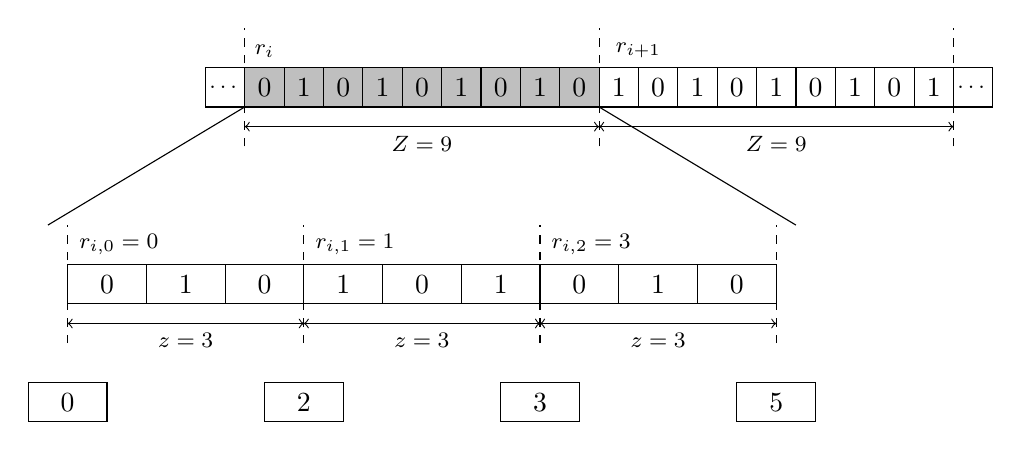
\begin{tikzpicture}[scale=0.5] % Adjust the scale as needed
            \foreach \x/\bit in {0/\footnotesize{\dots}, 1/0, 2/1, 3/0, 4/1, 5/0, 6/1, 7/0, 8/1, 9/0, 10/1, 11/0, 12/1, 13/0, 14/1, 15/0, 16/1, 17/0, 18/1, 19/\footnotesize{\dots}} {
                    \ifnum\x<1
                        \draw (\x,0) rectangle (\x+1,1) node[midway] {\bit};
                    \else
                        \ifnum\x<10
                            \draw[fill=lightgray] (\x,0) rectangle (\x+1,1) node[midway] {\bit};
                        \else
                            \draw (\x,0) rectangle (\x+1,1) node[midway] {\bit};
                        \fi
                    \fi
                }
            % Add dashed lines
            \draw[dashed] (1,-1) -- (1,2);
            \draw[dashed] (10,-1) -- (10,2);
            \draw[dashed] (19,-1) -- (19,2);

            % add double arrow
            \draw[<->] (1,-0.5) -- (10,-0.5) node[midway, below] {\footnotesize{$Z=9$}};
            \draw[<->] (10,-0.5) -- (19,-0.5) node[midway, below] {\footnotesize{$Z=9$}};

            % Add label over the blocks 2, 10
            \node[above] at (1.5,1) {\footnotesize{$r_i$}};
            \node[above] at (11,1) {\footnotesize{$r_{i+1}$}};

            % Add one line that starts from the bottom angle of block 1, and goes down inclined
            \draw[-] (1,0) -- (-4,-3);
            \draw[-] (10,0) -- (15,-3); % Adjusted target for second arrow

            \foreach \x/\bit in {0/0, 1/1, 2/0, 3/1, 4/0, 5/1, 6/0, 7/1, 8/0} {
                    \draw (\x*2-3.5,-5) rectangle (\x*2-1.5,-4) node[midway] {\bit};
                }

            % Add dashed lines
            \draw[dashed] (-3.5,-6) -- (-3.5,-3);
            \draw[dashed] (2.5,-6) -- (2.5,-3);
            \draw[dashed] (8.5,-6) -- (8.5,-3);
            \draw[dashed] (14.5,-6) -- (14.5,-3); % Adjusted target for second arrow line end point

            % add double arrow
            \draw[<->] (-3.5,-5.5) -- (2.5,-5.5) node[midway, below] {\footnotesize{$z=3$}};
            \draw[<->] (2.5,-5.5) -- (8.5,-5.5) node[midway, below] {\footnotesize{$z=3$}};
            \draw[<->] (8.5,-5.5) -- (14.5,-5.5) node[midway, below] {\footnotesize{$z=3$}};

            % Add label over the blocks 2, 10
            \node[above] at (-2.2,-4) {\footnotesize{$r_{i,0} = 0$}};
            \node[above] at (3.8,-4) {\footnotesize{$r_{i,1} = 1$}};
            \node[above] at (9.8,-4) {\footnotesize{$r_{i,2} = 3$}};


            \foreach \x/\bit in {-4.5/0, 1.5/2, 7.5/3, 13.5/5} { % Coordinates need adjustment if representing LUT
                    \draw (\x,-8) rectangle (\x+2,-7) node[midway] {\bit}; % Example values
                }
        \end{tikzpicture}
    \end{flushright}
    \caption{The hierarchical \textsf{rank} data structure. The first level is composed of superblocks of size $Z$ (conceptually storing absolute ranks $r_i$), the second level of blocks of size $z$ (storing relative ranks $r_{i,j}$), and the third level uses a lookup table (represented abstractly by the bottom row).} \label{fig:RRR}
\end{figure}


The lookup table $T$ allows determining the number of set bits within any prefix of a $z$-bit block in constant time. Table \ref{tab:lookup} shows an example for $z=3$. For a block $p$, the entry in column $j$ (corresponding to $\textsf{rank}_1(p, j)$) gives the precomputed result.

\begin{table}[h]
    \centering
    \begin{tabular}{|c|c|c|c|}
        % \hline
        %                & \multicolumn{3}{c|}{\textbf{cumulative rank at bit index}}                                           \\
        \hline
        \textbf{block} & $\mathbf{r_{i,0}}$ & $\mathbf{r_{i,1}}$ & $\mathbf{r_{i,2}}$ \\
        \hline
        000            & 0                  & 0                  & 0                  \\
        001            & 0                  & 0                  & 1                  \\
        010            & 0                  & 1                  & 1                  \\
        011            & 0                  & 1                  & 2                  \\
        100            & 1                  & 1                  & 1                  \\
        101            & 1                  & 1                  & 2                  \\
        110            & 1                  & 2                  & 2                  \\
        111            & 1                  & 2                  & 3                  \\
        \hline
    \end{tabular}
    \caption{Example of a lookup table $T$ for intra-block rank computation with $z = 3$. Each row corresponds to a possible $z$-bit pattern $p$. The cell for pattern $p$ and index $j$ stores $\textsf{rank}_1(p, j)$.} \label{tab:lookup}
\end{table}

We can state the following theorem regarding the space and time complexity \cite{Jacobson}.

\begin{theorem} \label{th:rank}
    Given a bitvector $B[1..n]$, there exists an auxiliary data structure using $o(n)$ bits that allows computing $\textsf{rank}_b(B, i)$ for any $i \in [1,n]$ and $b \in \{0,1\}$ in $O(1)$ time. The original bitvector $B$ is accessed only in read mode. The total space required is $n + o(n)$ bits.
\end{theorem}
\begin{proof}
    We construct the auxiliary data structure using a standard two-level hierarchical decomposition of the bitvector $B$. We define a \emph{superblock} size $Z = \lfloor \log^2 n \rfloor$ and a \emph{block} size $z = \lfloor (1/2) \log n \rfloor$. For analytical simplicity, assume $n$ is a multiple of $Z$, and $Z$ is a multiple of $z$.

    The structure comprises three main components designed to store precomputed rank information at different scales.

    First, the \emph{Superblock Rank Directory ($R_S$)} is an array storing the absolute rank at the start of each superblock. Specifically, for $k \in [0, n/Z - 1]$, $R_S[k] = \textsf{rank}_1(B, k \cdot Z)$. Since each rank value is at most $n$, storing these requires $\lceil \log n \rceil$ bits per entry. The total space for $R_S$ is:
    \begin{align*}
        \text{Space}(R_S) & = \frac{n}{Z} \lceil \log n \rceil = \frac{n}{\lfloor \log^2 n \rfloor} \lceil \log n \rceil \\
                          & = O\left(\frac{n \log n}{\log^2 n}\right) = O(n / \log n) \text{ bits}.
    \end{align*}

    Second, the \emph{Block Rank Directory ($R_B$)} stores ranks relative to the start of the containing superblock. For each block index $l \in [0, n/z - 1]$, let $k = \lfloor l \cdot z / Z \rfloor$ be its superblock index. $R_B[l]$ stores the relative rank $\textsf{rank}_1(B, l \cdot z) - \textsf{rank}_1(B, k \cdot Z)$. This value is at most $Z$, requiring $\lceil \log Z \rceil$ bits per entry. The total space for $R_B$ is:
    \begin{align*}
        \text{Space}(R_B) & = \frac{n}{z} \lceil \log Z = \frac{n}{\lfloor (1/2) \log n \rfloor} \lceil \log(\lfloor \log^2 n \rfloor) \rceil \\
                          & = O\left(\frac{n}{\log n} \log(\log^2 n)\right)                                                                   \\
                          & = O\left(\frac{n \log \log n}{\log n}\right) \text{ bits}.
    \end{align*}

    We verify that the space complexity for both directories $R_S$ and $R_B$ is sublinear, i.e., $o(n)$. For $R_S$, we have $O(n / \log n)$. As $n \to \infty$, $(n / \log n) / n = 1 / \log n \to 0$. For $R_B$, we have $O(n \log \log n / \log n)$. As $n \to \infty$, $(n \log \log n / \log n) / n = \log \log n / \log n \to 0$. Thus, both Space$(R_S)$ and Space$(R_B)$ are $o(n)$.

    Third, the \emph{Intra-Block Rank Mechanism ($T$)} is responsible for determining the rank within any $z$-bit block in constant time. A direct precomputation approach involves storing, for each of the $2^z$ possible $z$-bit patterns $p$ and each position $j \in [1, z]$, the value $\textsf{rank}_1(p, j)$. The space requirement for such a naive table would be:
    \[ \text{Space}(\text{Naive } T) = O(2^z \cdot z \cdot \log z). \]
    Substituting $z = \lfloor (1/2) \log n \rfloor$, this becomes
    \[ O(2^{(1/2)\log n} \log n \log \log n) = O(\sqrt{n} \log n \log \log n) \]
    which is not sublinear ($o(n)$). The crucial insight, originally provided by Jacobson \cite{Jacobson}, is that this intra-block rank functionality can indeed be implemented using auxiliary structures occupying only $o(n)$ bits while still supporting $O(1)$ query time. This often involves techniques like further table compression or specialized indexing strategies not detailed here, but whose existence and performance guarantees we rely upon.

    The total auxiliary space is the sum of the space complexities for $R_S$, $R_B$, and the efficient implementation of $T$. This sum is $O(n / \log n) + O(n \log \log n / \log n) + o(n)$, which simplifies to $o(n)$. Therefore, the total space including the original bitvector is $n + o(n)$ bits.
\end{proof}

It is worth noting a crucial optimization for practical implementations, especially when the block size $z$ is chosen such that it fits within a machine word (e.g., $z \le 64$ on standard 64-bit architectures). In this scenario, the theoretical $o(n)$-bit lookup mechanism $T$ for intra-block rank can often be replaced by direct computation using highly optimized hardware instructions.

Specifically, to compute the rank within the $z$-bit block $p = B[l \cdot z + 1 .. (l+1) \cdot z]$ up to position $j$, i.e., $\textsf{rank}_1(p, j)$, one can perform bitwise operations. First, isolate the $j$-bit prefix of $p$\footnote{For example, using a bitmask like $p \ \& \ ((1 \ll j) - 1)$}. Then, the number of set bits in this prefix can be computed efficiently using the processor's population count (popcount) instruction. Modern programming languages often expose this functionality directly; for instance, the Rust standard library provides the \texttt{count\_ones()} method on primitive integer types. This operation is typically executed in constant time (often a single machine instruction) and can be significantly faster in practice than accessing a more complex precomputed table structure, especially for small values of $z$.  We will discuss this in more detail in Section \ref{subsec:practical_considerations}.

To answer a query $\textsf{rank}_1(B, i)$, we perform the following constant-time steps:
Calculate the relevant indices: superblock $k = \lfloor (i-1)/Z \rfloor$, block $l = \lfloor (i-1)/z \rfloor$, and intra-block position $j = (i-1) \pmod z + 1$.
Retrieve the precomputed ranks: $rank_S = R_S[k]$ from the superblock directory and $rank_B = R_B[l]$ from the block directory.
Access the $z$-bit block $p = B[l \cdot z + 1 .. (l+1) \cdot z]$ from the original bitvector $B$. This access takes $O(1)$ time on a Word RAM where the word size $w \ge \log n \ge z$.
Compute the intra-block rank $rank_T = T(p, j)$ using the $o(n)$-space constant-time mechanism $T$.
The final rank is obtained by summing these components:
\[ \textsf{rank}_1(B, i) = rank_S + rank_B + rank_T. \]
All steps involve only constant-time operations (arithmetic, array lookups, memory access of $z$ bits, and the $T$ lookup), hence the total query time is $O(1)$.

The query $\textsf{rank}_0(B, i)$ is then computed simply as $i - \textsf{rank}_1(B, i)$, also in constant time.


% \subsection{Select} \label{subsec:select}
% The $select$ operation can be seen as the inverse of the rank operation, i.e given a binary array $B$ and an integer $i$, the $select$ operation returns the index of the $i$-th occurrence of a bit $b$ in $B$. More formally, we have that:
% \[
%     rank_c(B, select_c(B, i)) = i
% \]

% The implementation of the select operation heavily relies on the three level data structure discussed before (\ref{subsec:rank}). The difference lies in the fact that, in this case, the bitmap $B$ doesn't get split into blocks of fixed size, but rather into blocks of variable size that are determined by the rank of the block. We start by designing the first level of the select data structure: we split the bitmap $B$ into blocks of size $Z$ bitvectors each containing $K$ bits set to $1$.

% \begin{remark}[Notation and assumptions]
%     In the following, $Z$ will represent, as before, the size in bits of the big blocks containing $K$ bits set to $1$, where $K = \log n$. We will use always the same notation $Z$ even if the size of the blocks is variable, clarifying the context in which it is used.
% \end{remark}

% Since $K \leq Z$, we can easily derive that space occupance of all the starting positions of the blocks $O(\frac{n}{K} \log n) = o(n)$ bits. The first step of our search in then clear: since each block contains $K$ bits set to $1$, we can find the block containing the $i$-th occurrence of $1$ in $B$ by computing $i/K$.

% The second step is to find the $i$-th occurrence of $1$ in the block. This could be done by scanning the block from the beginning and counting the number of bits set to $1$ until we reach the $i$-th occurrence, but this would require $O(K)$ time making it highly un-efficient for our purposes. To address this issue, we introduce the second level of the select data structure where we divide the big blocks into smaller blocks and categorize them into two types: \emph{dense} and \emph{sparse} blocks. A big block is considered \emph{dense} if $Z \leq K^2$ and \emph{sparse} otherwise. When dealing with a sparse block, we can store the positions of the bits set to $1$ in the block in a separate array, allowing us to access the $i$-th occurrence of $1$ in constant time. Due to it's small number of bits set to $1$, we can store the positions in $O(\frac{n}{K^2}K \log n) = O(\frac{n}{\log^2n} \log n) = o(n)$ bits.

% Dealing with the dense blocks is not as straightforward as with the sparse ones. In this case, we can't afford to store the positions of the bits set to $1$ in the block, as it would require too much space. We introduce then the third level of the select data structure, where we split the dense blocks into smaller blocks of length\footnote{The same assumptions made before apply as well: $z$ can vary but we will use the same notation for simplicity and clarify the context in which it is used idf necessary} $z$, each containing $k = (\log \log m)^2$ bits set to $1$. Thus storing all the starting positions of the smalls blocks and relative beginning of the dense blocks requires $O(\frac{n}{k} \log K^2) = O(\frac{n}{(\log \log n)^2} \log \log^4 n) = o(n)$ bits\footnote{
%     We exploited the fact that each small block has at least length $k$ and the length of its enclosing dense block is at most $K^2$.
% }.

% The only remaining issue is to keep track of the positions of the bits set to $1$ in the small blocks. We can follow the idea introduced for the big blocks and divide them into \emph{dense} and \emph{sparse} small blocks. The sparse small blocks are those with length less then $k^2 = (\log \log m)^4$, and we can store the positions of the bits set to $1$ in the block relative to the beginning of its enclosing block in
% \[
%     O\left(\frac{n}{k^2} k \log K^2 \right) = O\left(\frac{n}{(\log \log n)^2} \log \log^4 n\right) = o(n)
% \]
% bits\footnote{
%     We exploited the fact that each sparse small block has length $z > k^2$, thus their number is $O(\frac{n}{k^2})$. We also note that the length of the enclosing dense block is at most $K^2$.
% }. Following the idea of the third level of the rank data structure, we can store the positions of the bits set to $1$ in the dense small blocks in a lookup table, allowing us to access the $i$-th occurrence of $1$ in constant time. This table will store all the pre-computed results of the select operation for all possible small blocks and, since $z \leq k^2$, having $2^z$ columns and $z$ rows, it will require $O(z 2^z \log z) = o(n)$ bits\footnote{
%     Each cell of the table stores a value in $[0, z]$, thus the $\log z$ factor.
% }.

% \begin{remark}[Pratical Considerations]
%     The value $(\log log m)^4$ can be very small for practical values of $m$, thus we could avoid dividing the small blocks into dense and sparse blocks and just scan the block from the beginning to find the $i$-th occurrence of $1$.
% \end{remark}

% In algorithm \ref{alg:select} are outlined the steps of the $select_1$ (the $select_0$ works in the same way) algorithm, which takes as input the binary array $B$ and an index $i$, and returns the index of the $i$-th occurrence of a bit $b$ in $B$.

% \begin{algorithm}[hbtp]
%     \caption{$Select_1$ Algorithm} \label{alg:select}
%     \begin{algorithmic}
%         \Function{$Select_1$}{$B, i$}
%         \State $ j = 1 + \lfloor \frac{i-1}{K} \rfloor$ \Comment{\small{index of big block}}
%         \State $B_{j} \gets$ big block $j$
%         \If{$B_{j}$ \emph{is sparse}}
%         \State $S \gets$ array of positions of bits set to $1$ in $B_{j}$
%         \State \Return $S[i \mod K]$
%         \Else
%         % the data structure has stored the staring position of the dense big block B_j, say s_j
%         \State $s_j \gets$ starting position of $B_{j}$
%         \State $i' \gets 1 + (i-1 \mod K)$ \Comment{\small{Relative $select$ index in the block}}
%         \State $j' \gets 1 + \lfloor \frac{i'-1}{k} \rfloor$ \Comment{\small{index of small block}}
%         \State $B_{j,j'} \gets$ small block $j'$ in big block $j$
%         % the data structure has stored the staring position of the dense small block B_{j,j'}, say s_{j,j'}
%         \State $s_{j,j'} \gets$ starting position of $B_{j,j'}$
%         \If{$B_{j,j'}$ \emph{is sparse}}
%         \State $S \gets$ array of positions of bits set to $1$ in $B_{j,j'}$
%         \State \Return $s_j + S[i' \mod k]$
%         \Else
%         % we access the lookup table T with values B_{j,j'} and 1 + (i+1 \mod k^2), and we get the answer to the select query by summig s_j + s_j' + T[B_{j,j'}, 1 + (i+1 \mod k^2)]
%         \State $o \gets 1 + (i'-1 \mod k^2)$ \Comment{\small{offset in the small block}}
%         \State \Return $s_j + s_{j,j'} + T[B_{j,j'}, o]$
%         \EndIf
%         \EndIf
%         \EndFunction
%     \end{algorithmic}
% \end{algorithm}

% As for the rank data structure, we can state the following theorem:

% \begin{theorem} \label{th:select}
%     The space occupancy of the Select data structure is $o(n)$ bits, and thus it is asymptotically sublinear in the size of the binary array $B[1, n]$. The Select algorithm takes constant time in the worst case, and accesses the array $B$ only in read-mode
% \end{theorem}
% \begin{proof}
%     Follows from the previous discussion.
% \end{proof}
% For dense small blocks whose size $z$ is very small (e.g., $z \le k^2 = (\log \log m)^4$), direct scanning can indeed be faster than accessing the precomputed table $T$.

\subsection{\textsf{Select}} \label{subsec:select}

The \textsf{select} operation serves as the inverse to \textsf{rank}. Formally, for a bitvector $B$ and an integer $i$, $\textsf{select}_b(B, i)$ returns the index $j$ such that $B[j] = b$ and $\textsf{rank}_b(B, j) = i$. This relationship can be expressed as:
\[ \textsf{rank}_b(B, \textsf{select}_b(B, i)) = i \]
provided the $i$-th occurrence of $b$ exists.

Supporting \textsf{select} queries efficiently requires a different auxiliary structure compared to the fixed-size blocking used for \textsf{rank}. An approach providing constant-time select within this space framework was developed by Clark \cite{clark1997compact}. It relies on a multi-level hierarchy guided by the number of set bits (specifically, 1s, as \textsf{select}$_0$ can be handled symmetrically or via \textsf{select}$_1$ on the complemented bitvector with additional rank structures). The core idea is to partition the bitvector $B$ based on the cumulative count of 1s and use multiple levels of indexing structures to locate the $i$-th 1 quickly.

We begin by designing the first level of the select data structure. The bitvector $B$ is conceptually divided into variable-length \emph{chunks}, such that each chunk (except possibly the last) contains exactly $K$ set bits. A typical choice is $K = \Theta(\log n \log \log n)$. We store an array $P_1$ containing the starting position (index in $B$) of each chunk. The number of chunks is $\lceil m/K \rceil$, where $m = \textsf{rank}_1(B, n)$ is the total number of 1s. The space for $P_1$ is
\[O(m/K \cdot \log n) = O(n / (\log n \log \log n) \cdot \log n) = O(n / \log \log n)\]
which is $o(n)$. Given a query $\textsf{select}_1(i)$, the relevant chunk index can be determined as $k = \lceil i/K \rceil$, and its starting position retrieved from $P_1$.

The second step addresses how to find the target 1 within its chunk. Let the length of a chunk be $Z$. We categorize chunks into two types based on their density. A chunk is considered \emph{sparse} if its length $Z$ is large compared to $K$, specifically $Z > K^2$. Conversely, a chunk is \emph{dense} if $Z \le K^2$. For sparse chunks, we can afford to store the relative positions (offsets from the chunk's start) of the $K$ set bits explicitly. The total space required across all sparse chunks for these offsets can be shown to be $o(n)$ \cite{clark1997compact}. If the target 1 falls within a sparse chunk, its position is found by calculating its relative rank $i' = (i-1) \pmod K + 1$ and retrieving the $i'$-th stored offset. For dense chunks ($Z \le K^2$), explicitly storing offsets is too costly. Instead, we introduce a second level of structure within these dense chunks.

This second level structure subdivides each dense chunk into smaller variable-length \emph{sub-chunks}, each containing exactly $k$ set bits, where $k = \Theta((\log \log n)^2)$. We store an array $P_2$ for each dense chunk, holding the starting positions of these sub-chunks relative to the start of the dense chunk. The total space for all $P_2$ structures across all dense chunks is $O(m/k \cdot \log Z_{max}) = O(n/k \cdot \log K^2) = O(n / (\log \log n)^2 \cdot \log(\log n \log \log n)) = o(n)$.

Finally, we need to handle the sub-chunks. Let a sub-chunk have length $z$. Similar to the chunk level, we distinguish between \emph{sparse sub-chunks} ($z > k^2$) and \emph{dense sub-chunks} ($z \le k^2$). For sparse sub-chunks, we again store the relative positions of the $k$ set bits explicitly; the total space across all sparse sub-chunks remains $o(n)$ \cite{clark1997compact}. For dense sub-chunks ($z \le k^2$), we require a mechanism to find the $i''$-th 1 (where $i''$ is the rank relative to the sub-chunk start) within the $z$ bits in constant time. It is known \cite{clark1997compact} that constant-time \textsf{select} within a block of size $z=O(\text{polylog } n)$ can be achieved using an auxiliary structure of size $o(z)$ bits associated with the block (e.g., using precomputed tables or other techniques). Summing over all dense sub-chunks, the total space for these Level 3 mechanisms is $o(n)$.

The overall query process involves navigating this hierarchy. The algorithm can be summarized by the following pseudocode.

\begin{algorithm}[hbtp]
    \caption{$Select_1$ Algorithm (Conceptual)} \label{alg:select}
    \begin{algorithmic}[1] \small
        \Function{$Select_1$}{$B, i$}
        \State $k \gets \lceil i/K \rceil$
        \State $pos_1 \gets \text{GetChunkStartPos}(k)$
        \State $ChunkInfo \gets \text{GetChunkInfo}(k)$
        \If{$ChunkInfo$ indicates \emph{sparse} ($Z > K^2$)}
        \State $i' \gets (i-1) \pmod K + 1$
        \State $offset \gets \text{GetSparseChunkOffset}(k, i')$
        \State \Return $pos_1 + offset$
        \Else
        \State $i' \gets (i-1) \pmod K + 1$
        \State $l \gets \lceil i'/k \rceil$
        \State $pos_2 \gets \text{GetSubChunkStartPos}(k, l)$
        \State $SubChunkInfo \gets \text{GetSubChunkInfo}(k, l)$
        \If{$SubChunkInfo$ indicates \emph{sparse} ($z > k^2$)}
        \State $i'' \gets (i'-1) \pmod k + 1$
        \State $offset \gets \text{GetSparseSubChunkOffset}(k, l, i'')$
        \State \Return $pos_1 + pos_2 + offset$
        \Else
        \State $i'' \gets (i'-1) \pmod k + 1$
        \State $offset \gets \text{DenseSubChunkSelect}(k, l, i'')$
        \State \Return $pos_1 + pos_2 + offset$
        \EndIf
        \EndIf
        \EndFunction
    \end{algorithmic}
\end{algorithm}

As for the rank data structure, we can state the following theorem:

\begin{theorem} \label{th:select}
    Given a bitvector $B[1..n]$, there exists an auxiliary data structure using $o(n)$ bits that allows computing $\textsf{select}_b(B, i)$ for any valid $i$ and $b \in \{0,1\}$ in $O(1)$ time. The original bitvector $B$ is accessed only in read mode. The total space required is $n + o(n)$ bits.
\end{theorem}
\begin{proof}
    The constant query time follows from the algorithm described, where each step (calculating indices, accessing pointer structures $P_1, P_2$, retrieving stored offsets for sparse cases, or using the constant-time Level 3 dense mechanism) takes $O(1)$ time. The total auxiliary space is the sum of the space required for $P_1$, the relative offsets for sparse chunks, the $P_2$ arrays, the relative offsets for sparse sub-chunks, the Level 3 dense sub-chunk mechanisms, and the structures needed to distinguish between sparse and dense cases. As analyzed during the description, each component requires $o(n)$ bits with parameters $K=\Theta(\log n \log \log n)$ and $k=\Theta((\log \log n)^2)$, relying on established results \cite{clark1997compact}. Therefore, the total auxiliary space is $o(n)$ bits, yielding an overall space of $n+o(n)$ bits.
\end{proof}

\begin{remark}[Practical Considerations]
    The threshold $k^2 = \Theta((\log \log n)^4)$ for handling the smallest dense blocks can be extremely small for practical values of $n$. In implementations, if $k$ is small enough (e.g., fits within a machine word or cache line), scanning the dense sub-chunk directly to find the $i''$-th occurrence of 1 might be faster than using the more complex theoretical $o(n)$ mechanism or precomputed tables. This again relates to broadword programming techniques, similar to the optimization mentioned for \textsf{rank}.
\end{remark}

\subsection{Compressing Sparse Bitvectors with Elias-Fano} \label{subsec:elias_fano_compression}

The rank and select structures discussed previously (\ref{subsec:rank}, \ref{subsec:select}) operate on the plain bitvector $B[1..n]$, achieving a total space occupancy of $n + o(n)$ bits. However, in many practical scenarios, the bitvector $B$ exhibits a skewed distribution, containing significantly fewer 1s than 0s (or vice-versa). Let $m = \textsf{rank}_1(B, n)$ be the total number of set bits. When $m \ll n$, storing the full $n$-bit vector is inefficient.

In such sparse settings, we can leverage compression techniques that exploit the low density of set bits. The Elias-Fano representation, previously introduced in Section~\ref{sec:elias_fano_code}, provides a highly effective method for this task. Recall that Elias-Fano encodes a monotonically increasing sequence of $m$ integers up to a maximum value $n$. We can represent the bitvector $B$ by encoding the sequence of indices $\{ i \mid B[i]=1 \}$.

As detailed by Vigna \cite{vigna2013quasi} in the context of quasi-succinct indices for information retrieval, the Elias-Fano representation achieves a space complexity of approximately $m \log_2(n/m) + O(m)$ bits. This is remarkably close to the information-theoretic lower bound for representing a subset of size $m$ from a universe of size $n$, often expressed as $n\mathcal{H}_0(B) + O(m)$ bits, where $\mathcal{H}_0(B)$ is the empirical zero-order entropy of the bitvector $B$. The crucial advantage is that the space depends primarily on $m$, the number of set bits, rather than the full length $n$, leading to significant compression when $m$ is small.

This compressed representation directly supports efficient operations. The $\textsf{select}_1(i)$ operation, finding the position of the $i$-th set bit, can typically be implemented in constant time on average, often leveraging auxiliary pointers within the Elias-Fano structure as engineered in \cite{vigna2013quasi}. However, this space efficiency comes at the cost of potentially slower $\textsf{rank}_1$ and accessing $B[i]$ operations compared to the $n+o(n)$ structures. These operations usually involve decoding parts of the Elias-Fano structure and may take $O(\log(n/m))$ time or depend on the specific implementation details \cite{navarro2016compact}. Therefore, Elias-Fano presents a compelling space-time trade-off, offering near-optimal compression for sparse bitvectors at the expense of $\textsf{rank}_1$ and access time complexity. The choice between plain bitvector structures and Elias-Fano depends critically on the sparsity of the data and the required query performance profile.

\subsection{Practical Implementation Considerations} \label{subsec:practical_considerations}

While the asymptotic analysis guarantees $O(1)$ query time and $o(n)$ extra space for the \textsf{rank} and \textsf{select} structures presented earlier, achieving high performance in practice requires careful consideration of architectural factors and constant overheads hidden in the $o(n)$ term. Memory latency, cache efficiency, and instruction-level parallelism often dominate the actual running time on modern processors.

A particularly effective approach for optimizing \textsf{rank} and \textsf{select} implementations leverages \emph{broadword programming} (also known as \textsc{Swar} - \textsc{Simd} Within A Register). This technique treats machine registers as small parallel processors, performing operations on multiple data fields packed within a single word using standard arithmetic and logical instructions. Vigna \cite{vigna2008broadword} applied these techniques to \textsf{rank} and \textsf{select} queries, leading to highly efficient practical implementations.

The \texttt{rank9} structure proposed by Vigna \cite{vigna2008broadword} exemplifies this approach. It employs a two-level hierarchy, similar in concept to the structure in Section~\ref{subsec:rank}, but critically relies on broadword algorithms for the final \textsf{rank} computation within a machine word (specifically, sideways addition or population count). Instead of large precomputed lookup tables for small blocks, \texttt{rank9} uses carefully designed constants and bitwise operations (detailed in Algorithm 1 of \cite{vigna2008broadword}) to compute the rank within a 64-bit word quickly. This typically involves storing relative counts for sub-blocks (e.g., seven 9-bit counts within a 64-bit word) in the second level. The advantages of this approach include speed, resulting from the exploitation of fast register operations and the avoidance of large table lookups, often outperforming other methods in practice. It also offers space efficiency, requiring relatively low overhead (typically around 25\% on top of the original bitvector $B$) mainly for the cumulative counts. Furthermore, broadword algorithms are generally branch-free, benefiting performance on modern pipelined processors by avoiding potential misprediction penalties.

Similarly, Vigna \cite{vigna2008broadword} developed broadword algorithms for selection within a word (Algorithm 2 in the paper). The companion \texttt{select9} structure integrates these intra-word selection capabilities with a multi-level inventory scheme. The objective of \texttt{select9} is to support high-performance selection queries, often achieving near constant-time execution, through hierarchical indexing combined with efficient broadword search for the final location. This capability involves an additional space cost, typically measured at approximately 37.5\% relative to the \texttt{rank9} structure.

Furthermore, a major bottleneck in \textsf{rank}/\textsf{select} operations is often memory access latency. To mitigate this, \emph{interleaving} the auxiliary data structures is highly recommended. For instance, storing a first-level (superblock) rank count immediately followed by its corresponding second-level (sub-block) counts increases the probability that all necessary auxiliary information for a query resides within the same cache line. This simple layout optimization can dramatically reduce cache misses compared to storing different levels of the hierarchy in separate arrays.
